%--------------------------------------------------------------------
% Reference manual, with description of the options
%--------------------------------------------------------------------
\chapter{Reference manual}
\label{c:3:refman}

We describe \safe commands and their basic usage.

\section{\safe commands}
One can run a \safe command as follows:
\begin{verbatim}
safe {command} [-{option}]*
     [-{phase}:{option}[={input}]]* {filename}+
\end{verbatim}
For example, the following command analyzes JavaScript code stored in a file name
``{sample.js}'' located in the current directory without showing detailed information
from the \verb!astRewriter! phase but printing the result of the \verb!cfgBuilder!
phase into a file name ``{out}'':
\begin{verbatim}
safe analyze -silent
             -cfgBuilder:out=out sample.js
\end{verbatim}

Each command has its own available options.  The most common options are as follows:
\begin{itemize}
\item \verb!-{phase}:silent!

\safe does not show messages during the phase.

\item \verb!-{phase}:out={out}!

\safe writes the result of the phase to a file \verb!out!.
% \item[\doption{-{phase}:out={out}}]: \\
%   \safe writes the result of the phase to a file name \verb!out!.
\end{itemize}
and the global options are \verb!-silent! and \verb!-testMode!.

The currently supported commands and their options are as follows:
\begin{itemize}
\item \verb!parse -parser:out={out}!

parses the JavaScript code in a given file.
\item \verb!astRewrite -astRewriter:silent!\\
\hspace*{5.8em}\verb!-astRewriter:out={out}!

generates a simplified Abstract Syntax Tree (AST)
of the  JavaScript code in a given file.
\item \verb!compile -compiler:silent!\\
\hspace*{4.2em}\verb!-compiler:out={out}!

generates an Intermediate Representation (IR)
of the  JavaScript code in a given file.
\item \verb!cfgBuild -cfgBuilder:silent!\\
\hspace*{4.8em}\verb!-cfgBuilder:out={out}!\\
\hspace*{4.8em}\verb!-cfgBuilder:dot={name}!

generates a Control Flow Graph (CFG) of the  JavaScript code in a given file.

If \verb!-cfgBuilder:dot=name! is given,
\safe writes the resulting CFG in a graph visualization format
to file names \verb!name.gv! and \verb!name.pdf!.

\item \verb!analyze -analyzer:silent!\\
\hspace*{4.4em}\verb!-analyzer:out={out}!\\
\hspace*{4.4em}\verb!-analyzer:console!\\
\hspace*{4.4em}\verb!-analyzer:html={name}!

analyzes the  JavaScript code in a given file.

If \verb!-analyzer:console! is given,
\safe enables a user to debug analysis results by investigating the intermediate
status of the analysis.

If \verb!-analyzer:html=name! is given,
\safe writes the resulting CFG with states that can be investigated to
file name \verb!name.html!.

We describe these facilities in the next section.

\item \verb!help! shows the usage of \safe commands to the standard output.
\end{itemize}

\medskip
The \verb!parse! command parses the JavaScript code in a given file and
rewrites obvious dynamic code generation into other statements without using
dynamic code generation but with the same semantics.  For example, the following
JavaScript code
\begin{verbatim}
function f() { return 3; }
eval("f()")
\end{verbatim}
is rewritten as follows:
\begin{verbatim}
function f() { return 3; }
f();
\end{verbatim}

\medskip
The \verb!astRewrite! command parses the JavaScript code in a given file and
rewrites its AST representation into a simpler AST.
The \verb!astRewriter! phase performs three kinds of AST transformations:
\begin{itemize}
\item \verb!Hoister! lifts the declarations of functions and variables inside
programs and functions up to the beginning of them.
\item \verb!Disambiguator! checks some static restrictions and renames identifiers
to unique names.
\item \verb!WithRewriter! rewrites the \verb!with! statements that do not include
any dynamic code generation such as \verb!eval! into other statements without using
the \verb!with! statement but with the same semantics~\cite{dls13,withtr}.
\end{itemize}

Note that building a graph visualization format of CFGs requires the \verb!dot! program
from Graphviz~\cite{graphviz} be in your path.
For example, the following command:
\begin{verbatim}
safe cfgBuild -cfgBuilder:dot=dot sample.js
\end{verbatim}
runs the following command:
\begin{verbatim}
dot -Tpdf dot.gv -o dot.pdf
\end{verbatim}
to produce something like the following:
\begin{figure}[H]
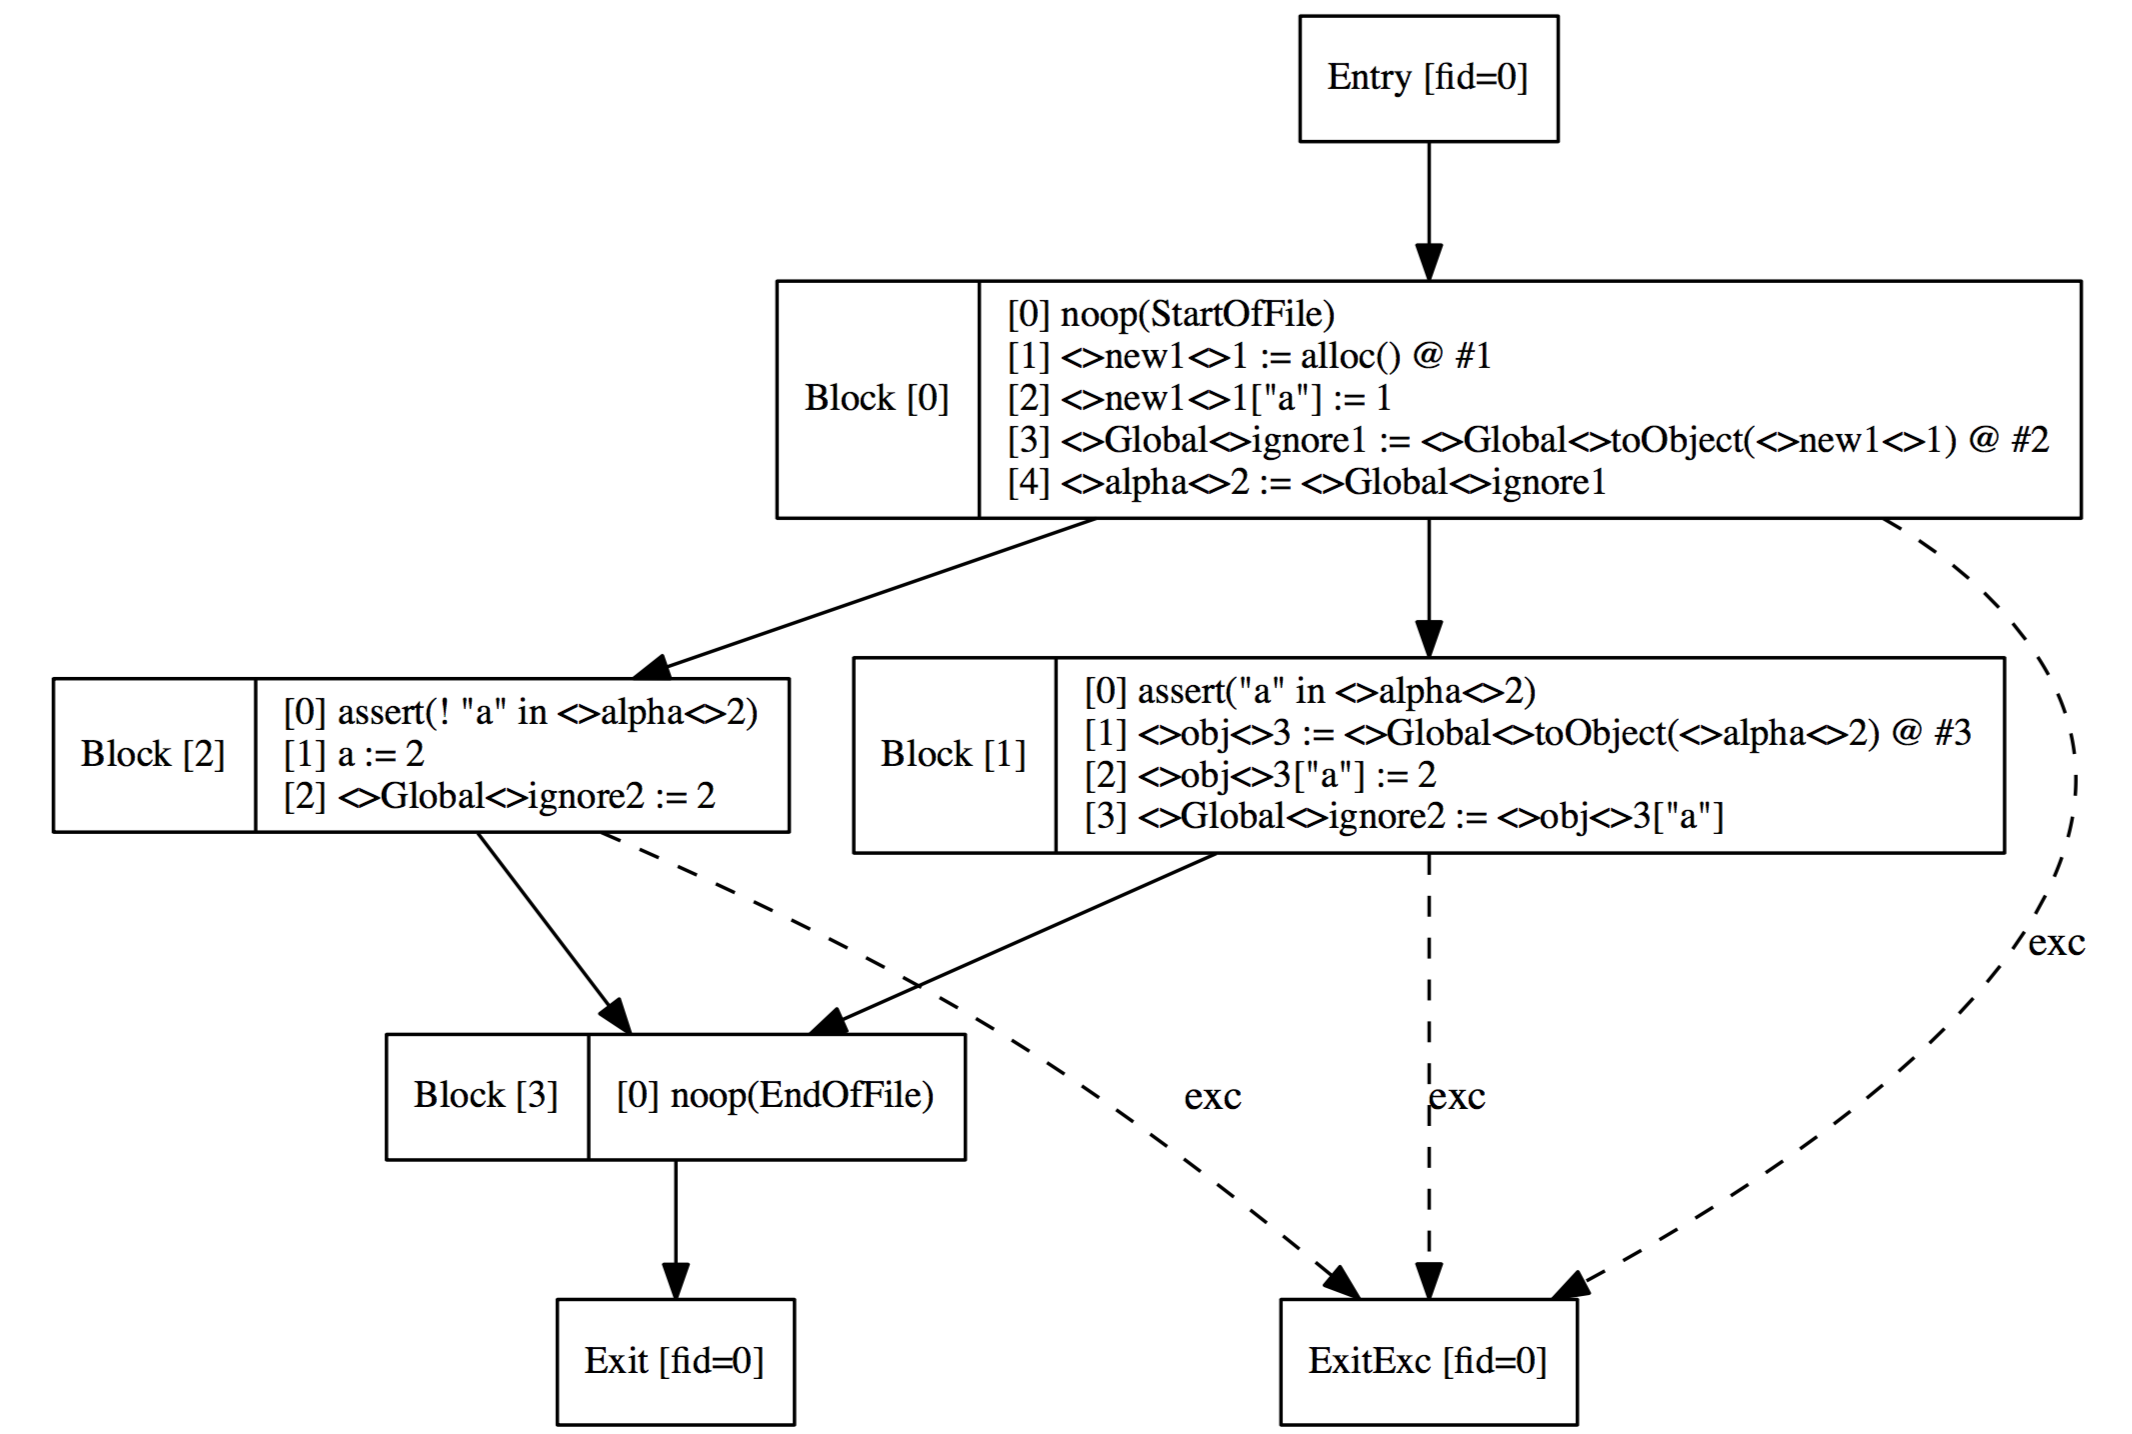
\includegraphics[width=8.75cm]{cfg.png}
\end{figure}

\section{\safe analyzer debugging}
When the \verb!-analyzer:console! option is given to the \texttt{analyze} command,
\safe provides a REPL-style console debugger.
For example, the following command:
\begin{verbatim}
safe analyze -analyzer:console test.js
\end{verbatim}
shows the list of available commands for debugging and
the starting point of the analysis:
{\small
\begin{verbatim}
Command list:
- help           
- next       jump to the next iteration. (same as "")
- jump       Continue to analyze until the given
             iteration.
- print      Print out various information.
- result     Print out various information.
- run_insts  Run instruction by instruction.
- move       Change a current position.
- home       Reset the current position.
- run        Run until meet some break point.
- break      Add a break point.
- break-list Show the list of break points.
- break-rm   Remove a break point.
For more information, see 'help <command>'.

<function[0] top-level: Entry[-1], ()> @test.js:1:1
Iter[0] > 
\end{verbatim}
}

The current status is denoted as follows:
{\small
\begin{verbatim}
<function [{fid}] {fun-name}: {block-kind}[{bid}],
 {call-context}> @{filename}:{span}
Iter[{#iteration}] >
\end{verbatim}
}
\noindent
where \verb!fid! and \verb!fun-name! are the id and the name of the current function,
respectively, \verb!block-kind! and \verb!bid!
are the kind and the id of the current block, respectively,
\verb!call-context! is the call context of the current analysis,
\verb!filename! is the name of the file being analyzed,
\verb!span! is the location of the current analysis, and
\verb!#iteration! is the iteration number of the current analysis.

A block is one of the following kinds:
\begin{itemize}
\itemsep-.1em
\item Entry: the entry block of a function
\item Block: a normal block with instructions
\item Exit: the exit block of a function
\item ExitExc: a block denoting uncaught exceptions in a function
\item Call: a block denoting a function call
\item AfterCall: a block receiving a return value of a function call
\item AfterCatch: a block receiving uncaught exceptions after a function call
\item ModelBlock: a block denoting a modeled function
\end{itemize}

The \verb!help! command displays a list of available commands and
the \verb!help <command>! command displays the usage of the \verb!<command>!.
For example:
{\small
\begin{verbatim}
<function[0] top-level: Entry[-1], ()> @test.js:1:1
Iter[0] > help print
usage: print state(-all) ({keyword})
       print block
       print loc {LocName} ({keyword})
       print func {functionID}
       print worklist
       print ipsucc
       print trace
       print cfg
\end{verbatim}
}
\noindent
shows the usage of the \verb!print! command.

\medskip
The \verb!next! command proceeds the analysis of the current block,
which is the default command.  For example:
{\small
\begin{verbatim}
<function[0] top-level: Entry[-1], ()> @test.js:1:1
Iter[0] >

<function[0] top-level: Block[0], ()> @test.js:1:1-7:18
Iter[1] >
\end{verbatim}
}

\medskip
The \verb!jump {#iteration}! command proceeds the analysis until the given
number of iterations.  For example:
{\small
\begin{verbatim}
<function[0] top-level: Entry[-1], ()> @test.js:1:1
Iter[0] > jump 10

<function[0] top-level: Block[4], ()> @test.js:7:5-21:1
Iter[10] >
\end{verbatim}
}

\medskip
The \verb!print! command displays the status just before
analyzing the current block.  We describe it in Section~\ref{s:3:2:1:refman}.

\medskip
The \verb!result! command displays the status after analyzing
the current block:
\begin{itemize}
\item \verb!result (exc-)state(-all) ({keyword})!

It displays the state in the same way as the \verb!print! command does,
and it can additionally show the exception state generated after the analysis.
\item \verb!result (exc-)loc {LocName}!

It finds and displays the location in the same way as the \verb!print! command does,
and it can additionally find and display the location from
the exception state generated after the analysis.
\end{itemize}

\medskip
The \verb!run_insts! command shows the list of instructions in the current block,
and it enables to analyze each instruction.  It opens a sub-console, which provides 3 kinds
of commands:
\begin{itemize}
\itemsep-.1em
\item \verb!s! shows the state
\item \verb!q! quits the analysis
\item \verb!n! analyzes the next instruction; the default command
\end{itemize}
For example:
{\small
\begin{verbatim}
<function[0] top-level: Block[4], ()> @test.js:8:5-26:1
Iter[10] > run_insts 
Block[4] -> Exit, ExitExc
  [0] shift := <>Global<>ignore6
  [1] __result1 := shift !== "x"
  [2] __expect1 := false
  [3] <>obj<>10 := <>Global<>toObject(obj) @ #13
  [4] __result2 := <>obj<>10["length"] !== 1
  [5] __expect2 := false
  [6] <>obj<>11 := <>Global<>toObject(obj) @ #14
  [7] __result3 := <>obj<>11[0] !== "y"
  [8] __expect3 := false
  [9] <>obj<>12 := <>Global<>toObject(obj) @ #15
  [10] __result4 := <>obj<>12[1] !== undefined
  [11] __expect4 := false
  [12] noop(EndOfFile)

inst: [0] shift := <>Global<>ignore6
('s': state / 'q': stop / 'n','': next)
>

inst: [1] __result1 := shift !== "x"
('s': state / 'q': stop / 'n','': next)
> 
\end{verbatim}
}

\medskip
The \verb!move {fid}:{{bid}|entry|exit|exitExc}! command
moves the current block to the given block denoted by the id of a function,
the id of a block, and the kind of the block.  For example:
{\small
\begin{verbatim}
<function[0] top-level: ExitExc[-3], ()> @test.js:26:1
Iter[12] > move 0:exit
* current control point changed.

<function[0] top-level: Exit[-2], ()> @test.js:26:1
Iter[12] >
\end{verbatim}
}

\medskip
The \verb!home! command moves the current block back to the original
block to be analyzed.  For example:
{\small
\begin{verbatim}
<function[0] top-level: Exit[-2], ()> @test.js:26:1
Iter[12] > home
* reset the current control point.

<function[0] top-level: ExitExc[-3], ()> @test.js:26:1
Iter[12] >
\end{verbatim}
}

\medskip
The \verb!run! command proceeds the analysis until encountering a break
point.  A short-key for this command is Ctrl-d.  For example:
{\small
\begin{verbatim}
<function[0] top-level: Entry[-1], ()> @test.js:1:1
Iter[0] > break 0:exit

<function[0] top-level: Entry[-1], ()> @test.js:1:1
Iter[0] > run

<function[0] top-level: Exit[-2], ()> @test.js:26:1
Iter[11] >
\end{verbatim}
}

\medskip
The \verb!break! command sets up a break point at the given block.
For example:
{\small
\begin{verbatim}
<function[0] top-level: Entry[-1], ()> @test.js:1:1
Iter[0] > break 0:exit

<function[0] top-level: Entry[-1], ()> @test.js:1:1
Iter[0] > run

<function[0] top-level: Exit[-2], ()> @test.js:26:1
Iter[11] >
\end{verbatim}
}

\medskip
The \verb!break-list! command shows a list of blocks with
break points.  For example:
{\small
\begin{verbatim}
<function[0] top-level: Exit[-2], ()> @test.js:26:1
Iter[11] > break-list
* 2 break point(s).
  [0] function[0] Exit[-2]
  [1] function[0] Entry[-1]
\end{verbatim}
}

\medskip
The \verb!break-rm {break-order}! command
removes the break point of a given block
denoted by the order in the result of \verb!break-list!.
For example:
{\small
\begin{verbatim}
<function[0] top-level: Exit[-2], ()> @test.js:26:1
Iter[11] > break-list
* 2 break point(s).
  [0] function[0] Exit[-2]
  [1] function[0] Entry[-1]

<function[0] top-level: Exit[-2], ()> @test.js:26:1
Iter[11] > break-rm 0
* break-point[0] removed.
[0] function[0] Exit[-2]

<function[0] top-level: Exit[-2], ()> @test.js:26:1
Iter[11] > break-list
* 1 break point(s).
  [0] function[0] Entry[-1]
\end{verbatim}
}

\subsection{Analyzer debugging with printing}
\label{s:3:2:1:refman}
The \verb!print! command displays the status just before
analyzing the current block.

\medskip\noindent
\fbox{\texttt{print state(-all) (\{keyword\})}}\\[.2em]
The \verb!print state! command displays the current state,
and the \verb!print state-all! command
displays the current state including all system addresses.
When a keyword is given, it displays only the parts that include the keyword.
For example:
{\small
\begin{verbatim}
<function[0] top-level: Exit[-2], ()> @test.js:21:1
Iter[12] > print state result
           "__result1" -> [ttf] false
           "__result2" -> [ttf] false
           "__result3" -> [ttf] false
           Set(NaN, __result3, Function,
__EvalErrLoc, URIError, pop, JSON, Error, Number,
decodeURIComponent, __SyntaxErrProtoLoc, RangeError,
__RangeErrLoc, __ArrayConstLoc, __EvalErrProtoLoc,
Boolean, ReferenceError, __RefErrLoc, obj, __BOT,
encodeURIComponent, __TypeErrProtoLoc, Array,
EvalError, __expect1, encodeURI, eval, __expect3,
isFinite, __ErrProtoLoc, Object, __TOP, Math,
__TypeErrLoc, __URIErrProtoLoc, __result1,
parseFloat, __RangeErrProtoLoc, TypeError,
<>Global<>global, __ObjConstLoc, isNaN, __URIErrLoc,
Date, __NumTop, __expect2, decodeURI, RegExp,
__BoolTop, __UInt, parseInt, __result2, __StrTop,
Infinity, SyntaxError, __RefErrProtoLoc, __Global,
<>Global<>true, __SyntaxErrLoc, undefined, String)
\end{verbatim}
}

\medskip\noindent
\fbox{\texttt{print block}}\\[.2em]
The \verb!print block! command displays the information of
a given block.  For example:
{\small
\begin{verbatim}
<function[0] top-level: Block[0], ()> @test.js:1:1-7:18
Iter[1] > print block
Block[0] -> [1], ExitExc
  [0] noop(StartOfFile)
  [1] <>Global<>ignore1 := alloc() @ #1
  [2] obj := <>Global<>ignore1
  [3] <>obj<>1 := <>Global<>toObject(obj) @ #2
  [4] <>obj<>2 := <>Global<>toObject(Array) @ #3
  [5] <>obj<>3 :=
      <>Global<>toObject(<>obj<>2["prototype"]) @ #4
  [6] <>obj<>1["pop"] := <>obj<>3["pop"]
  [7] <>obj<>4 := <>Global<>toObject(obj) @ #5
  [8] <>obj<>4[4294967294] := "x"
  [9] <>obj<>5 := <>Global<>toObject(obj) @ #6
  [10] <>obj<>5["length"] := - 1
  [11] <>obj<>6 := <>Global<>toObject(obj) @ #7
  [12] <>arguments<>7 := allocArg(0) @ #8
  [13] <>fun<>8 :=
       <>Global<>toObject(<>obj<>6["pop"]) @ #9
\end{verbatim}
}

\medskip\noindent
\fbox{\texttt{print loc \{LocName\} (\{keyword\})}}\\[.2em]
The \verb!print loc {LocName}! command shows the object
bound at a given location in the current state.
When a keyword is given, it displays only the parts that include the keyword
in the object.  For example:
{\small
\begin{verbatim}
<function[0] top-level: ExitExc[-3], ()> @test.js:21:1
Iter[12] > print loc #1
#1 -> [[Class]] : "Object"
      [[Extensible]] : true
      [[Prototype]] : #Object.prototype
      "4294967294" -> [ttt] "x"
      "length" -> [ttt] -1
      "pop" -> [ttt] #Array.prototype.pop
      Set(pop, length, 4294967294)
\end{verbatim}
}

\medskip\noindent
\fbox{\texttt{print func (\{functionID\})}}\\[.2em]
It displays the list of functions.
If a function id is given, it displays the name and the span of it.
For example:
{\small
\begin{verbatim}
<function[0] top-level: ExitExc[-3], ()> @test.js:21:1
Iter[12] > print func 0
* function name: top-level
* span info.   : test.js:1:1-21:1
\end{verbatim}
}

\medskip\noindent
\fbox{\texttt{print worklist}}\\[.2em]
It shows the work in the current worklist.  For example:
{\small
\begin{verbatim}
<function[42] []Array.prototype.pop: ExitExc[-3],
 (10)> @[]Array.prototype.pop:0:0
Iter[6] > print worklist
* Worklist set
(42:ExitExc[-3], (10)), (42:Exit[-2], (10)),
(0:AfterCall[2], ()), (0:ExitExc[-3], ())
\end{verbatim}
}

\medskip\noindent
\fbox{\texttt{print ipsucc}}\\[.2em]
It displays the information of the current inter-procedural successor.
For example:
{\small
\begin{verbatim}
<function[42] []Array.prototype.pop: ExitExc[-3],
 (10)> @[]Array.prototype.pop:0:0
Iter[6] > print ipsucc
* successor map
- src: FlowSensitiveCP(ExitExc[-3],(10))
- dst: FlowSensitiveCP(AfterCatch[3],()),
 mayOld: (10, 1, 8)
mustOld: (10, 1, 8)
\end{verbatim}
}

\medskip\noindent
\fbox{\texttt{print trace}}\\[.2em]
It shows the current call trace.  For example:
{\small
\begin{verbatim}
<function[42] []Array.prototype.pop: Entry[-1],
 (10)> @[]Array.prototype.pop:0:0
Iter[3] > print trace
* Call-Context Trace
Entry[-1] of function[42] []Array.prototype.pop with (10)
 1>  [0] call(<>fun<>8, <>obj<>6, <>arguments<>7) @ #10
test.js:7:11-20 @Call[1] of function[0] top-level with ()
\end{verbatim}
}

\medskip\noindent
\fbox{\texttt{print cfg \{name\}}}\\[.2em]
It prints the current CFG to files \verb!name.gv! and \verb!name.pdf!.

\medskip\noindent
\fbox{\texttt{print html \{name\}}}\\[.2em]
It prints the current CFG and its state to the \verb!name.html! file.
We describe this facility in the next section.

\subsection{Analyzer debugging with browsing}
\label{s:3:2:2:refman}
The \verb!print html! command writes the current status into an HTML file
so that a user can investigate the analysis status from a browser.
Consider the following snapshot:
\begin{figure}[H]
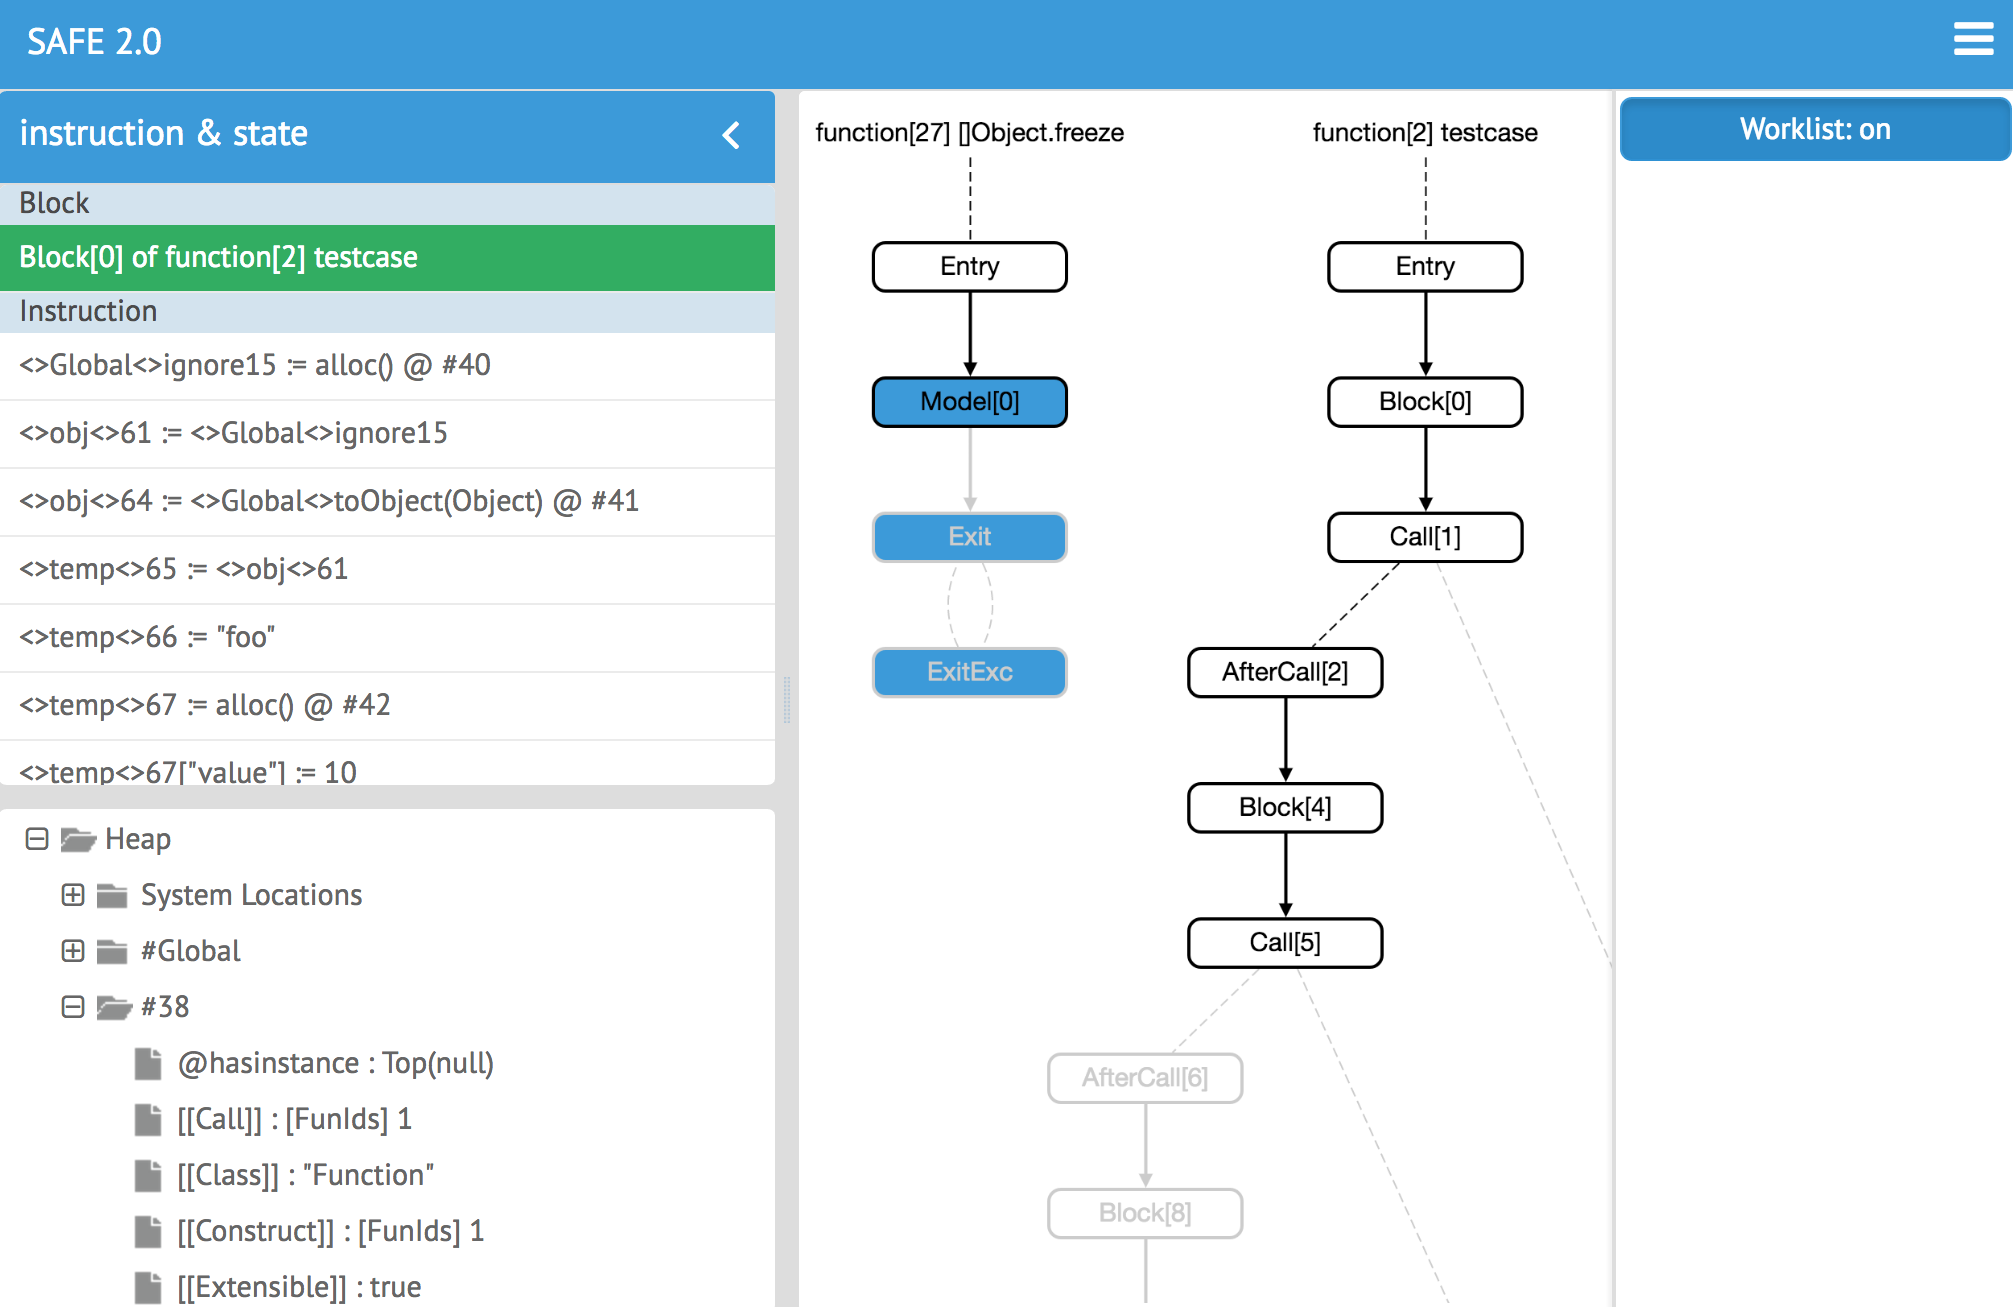
\includegraphics[width=8.75cm]{htmldebugger.png}
\end{figure}
\noindent
which shows the current CFG in the middle.
Nodes in black lines denote the blocks that are analyzed,
those in gray lines denote the blocks not yet being analyzed, and
colored nodes denote the blocks that are currently in the worklist of the analyzer.
One can toggle whether to show the nodes in the worklist by the menu button on the top right.
When a user selects a block from the CFG, the list of the instructions in the block
and the state just before analyzing the block are displayed on the left.
